%%%%%%%%%%%%%%%%%%%%%%%%%%%%%%%%%%%%%%%%%%%%%%%%%%%%%%%%%%%%%%%%%%%%%%%%%%%
%
% Template for a LaTex article in English.
%
%%%%%%%%%%%%%%%%%%%%%%%%%%%%%%%%%%%%%%%%%%%%%%%%%%%%%%%%%%%%%%%%%%%%%%%%%%%

\documentclass{article}

% AMS packages:
\usepackage{amsmath, amsthm, amsfonts}
\usepackage{algorithm}
\usepackage[noend]{algpseudocode}
\usepackage{graphicx}
\graphicspath{ {images/} }

% Theorems
%-----------------------------------------------------------------
\newtheorem{thm}{Theorem}[section]
\newtheorem{cor}[thm]{Corollary}
\newtheorem{lem}[thm]{Lemma}
\newtheorem{prop}[thm]{Proposition}
\theoremstyle{definition}
\newtheorem{defn}[thm]{Definition}
\theoremstyle{remark}
\newtheorem{rem}[thm]{Remark}

\makeatletter
\def\BState{\State\hskip-\ALG@thistlm}
\makeatother

% Shortcuts.
% One can define new commands to shorten frequently used
% constructions. As an example, this defines the R and Z used
% for the real and integer numbers.
%-----------------------------------------------------------------
\def\RR{\mathbb{R}}
\def\ZZ{\mathbb{Z}}

% Similarly, one can define commands that take arguments. In this
% example we define a command for the absolute value.
% -----------------------------------------------------------------
\newcommand{\abs}[1]{\left\vert#1\right\vert}

% Operators
% New operators must defined as such to have them typeset
% correctly. As an example we define the Jacobian:
% -----------------------------------------------------------------
\DeclareMathOperator{\Jac}{Jac}

%-----------------------------------------------------------------
\title{Vector Field Based Shape Deformations Note}
\author{ShengweiZHANG\\
  %% \small Dept. Templates and Editors\\
  %% \small E12345\\
  %% \small Spain
}

\begin{document}
\maketitle

%% \abstract{Compiling Embedded\_thin\_shell progress}

\section{Abstract}
The paper construct a $C^1$ continuous, divergence-free vector field to deform a 3d model.
\section{The Vector Field}
In 3D, a divergence-free vector field $v$ can be constructed from the gradients of two scalar fields $p(x,y,z), q(x,y,z)$ as
\begin{equation}
  v(x,y,z) = \nabla p \times \nabla q
\end{equation}
which in other words, v is constructed by the cross product of two divergence-free vector field $\nabla p$ and $\nabla q$.
In this paper we seprate the model into three parts: \textit{inner region}, \textit{outer region} and \textit{blended region} and using a piecewise linear vector field to deform the 3d model.
The points in the \textit{inner region} are fully deformed, the points in the \textit{outer region} are no deform, and the points in the \textit{blended region} are blended deformed.
The scalar field p,q are defined as:
\begin{equation}
  p(x,t)=\begin{cases} e(x,t) & \mbox{ } r(x)<r_i\\
  (1-b)\cdot e(x,t) + b \cdot 0 &\mbox{ } r_i \le r(x) < r_o\\
  0 &  \mbox{ } r_o \le r(x) \end{cases}
\end{equation}
\begin{equation}
  q(x,t)=\begin{cases} f(x,t) & \mbox{ } r(x)<r_i\\
  (1-b)\cdot f(x,t) + b \cdot 0 &\mbox{ } r_i \le r(x) < r_o\\
  0 &  \mbox{ } r_o \le r(x) \end{cases}\\
\end{equation}
by a scalar field $r(x)$ we separate the three parts, and v is blended by the blending function $b=b(r(x))$ in the \textit{blended region}. b is defined by B́ezier representation\footnote{\noindent B́ezier representation $B_n(f)=\sum\limits_{k=0}^n \left(\begin{array}{c} n\\k \end{array}\right)x^k(1-x)^{n-k} f(\frac{k}{n})$. $B_n(f)(x) \rightarrow f(x)$ \\as $n\rightarrow \infty$.}:
\begin{equation}
  b(r) = \sum\limits_{i=0}^4 w_i B_i^4(\frac{r-r_i}{r_o-r_i})
\end{equation}
here let $w_0 = w_1 = w_2 = 0$ and $w_3 = w_4 = 1$\footnote{\noindent see Bezier Representation.}.
Then the vector field should be:
\begin{equation}
 \nabla p(x,t) = \begin{cases} \nabla e(x,t) & \mbox{ } r(x) <r_i\\
   [-\nabla b \cdot e(x,t) + (1-b) \nabla e(x,t)] \times [-\nabla b \cdot f(x,t) + (1-b) \nabla f(x,t)] & \mbox{ } r_i \le r(x) < r_o\\
   0 & \mbox{ } r_o \le r(x) \end{cases}
\end{equation}
\begin{equation}
 \nabla p(x,t) = \begin{cases} \nabla e(x,t) & \mbox{ } r(x) <r_i\\
   [-\nabla b \cdot e(x,t) + (1-b) \nabla e(x,t)] \times [-\nabla b \cdot f(x,t) + (1-b) \nabla f(x,t)] & \mbox{ } r_i \le r(x) < r_o\\
   0 & \mbox{ } r_o \le r(x) \end{cases}
\end{equation}

\section{Integration}
\begin{equation}
  x_{k+1} = \int_{t_k}^{t_{k+1}} v(x_t, t) dt + x_k
\end{equation}

\begin{algorithm}
\caption{Integrator algorithm}\label{euclid}
\begin{algorithmic}
 \Procedure{Init Procedure}{}
\State $\textit{h} \gets $\textit{T/time\_slice}
\State $i \gets \textit{0}$
\State $cur\_t \gets \textit{init\_time}$
\EndProcedure
 \For{{$\textit{i} < $\textit{time\_slice}}}
 \State $\textit{construct vector field v}$
 \State$x = funcAdv(v(x,cur\_t)) + x$
 \State$cur\_t += h$
\EndFor
\end{algorithmic}
\end{algorithm}

\section{Implicit tools}
\subsection{Sphere Deform Tool}
Construst a constant vector field in the inner region $\textbf{v}=(u, v, w)$, where $\textbf{v}$ is the translation of the sphere's center, for that target choose two orthogonal vectors: $\textbf{u}$ and $\textbf{v}$, which $\textbf{u} \times \textbf{v} = \textbf{v}$. Then e(x) and f(x) is:
\begin{equation}
  e(x)=\textbf{u}(\textbf{x}-\textbf{c}), f(x)=\textbf{w}(\textbf{x}-\textbf{c})
\end{equation}
where $\textbf{c}$ is the current center. The region function is defined as
\begin{equation}
  r(\textbf{x}) = (\textbf{x}-\textbf{c})^2
\end{equation}
\subsection{Bending Deform Tool}
A linear vector field v is used to describe a rotation inside the inner region. Given a rotational axis by a center point $\textbf{c}$ and the normalized axis direction $\textbf{a}$, Then the e(x) and f(x) is:
\begin{equation}
  e(x) = \textbf{a}(\textbf{x}-\textbf{c}), f(x)= (\textbf{a} \times (\textbf{x} - \textbf{c}))^2
\end{equation}
from quation up, we can derive that the angular velocity in the inner region is 2, take $Line(\textbf{a} , \textbf{c})$ as axis.\footnote{\noindent see Appendix.}
The region function is defined as
\begin{equation}
  r(\textbf{x}) = \textbf{b} \cdot (\textbf{x}-\textbf{c})
\end{equation}
Innfer from the paper, $\textbf{b}$ rotate the half of the inner regions rotation. So in each time\_step update $\textbf{b}$ and recaculate r(x) and update vector field.
\begin{equation}
  \textbf{b} = rotate\_mat * \textbf{b}
\end{equation}
\subsection{Twist Deform Tool}
By using a linearly increasing rotation defined by:
\begin{equation}
e(x) = (a \cdot (x-c) )^2,  f(x)=(a \times (x-c) )^2
\end{equation}
 we construct a twist vector field in the inner region.\footnote{\noindent we can construct a more understanble scalar field e(x), see Appendix}
 \begin{figure}[H]
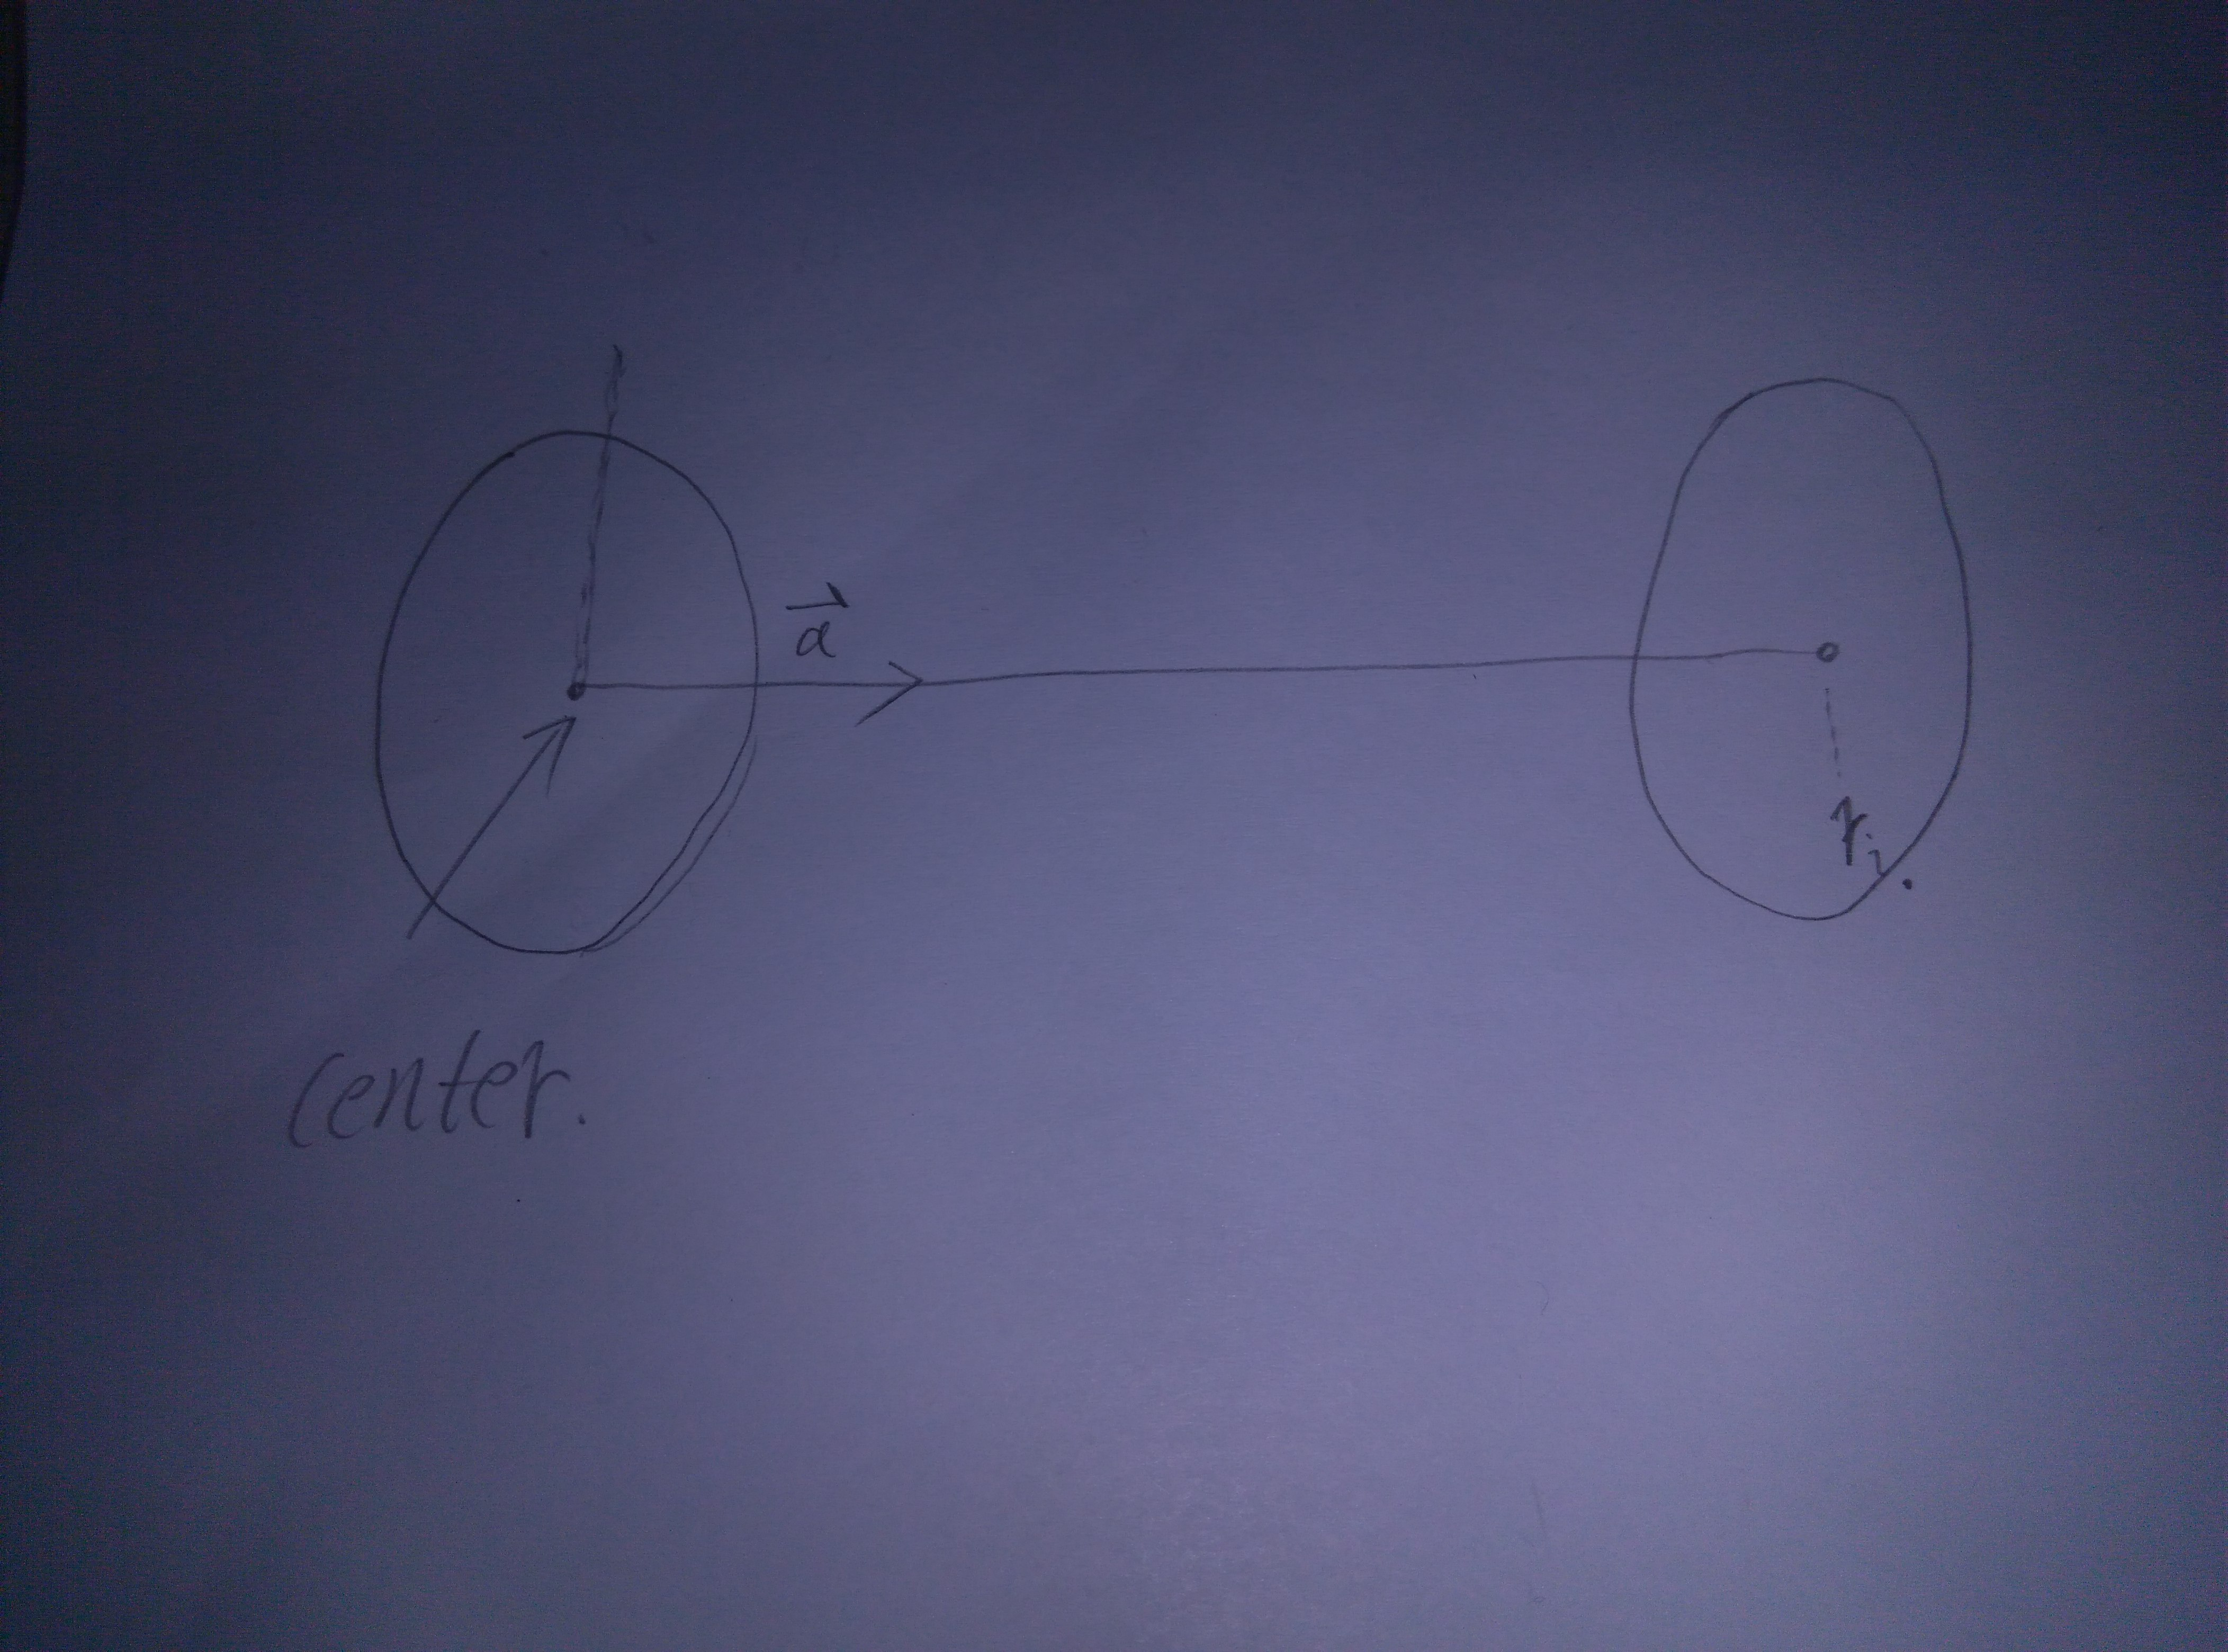
\includegraphics[width=8cm]{twist}
\centering
\end{figure}
The region function is defind as:
\begin{equation}
  r(x) = a \cdot (x-c)
\end{equation}

\section{Result}
Sphere Deform Tool:
\begin{figure}[H]
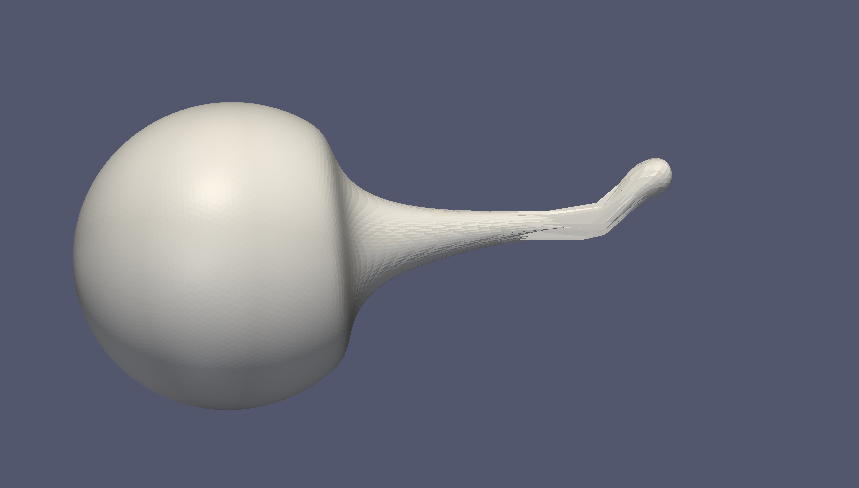
\includegraphics[width=8cm]{sphere_deform_result}
\centering
\end{figure}

Bend Deform Tool:
\begin{figure}[H]
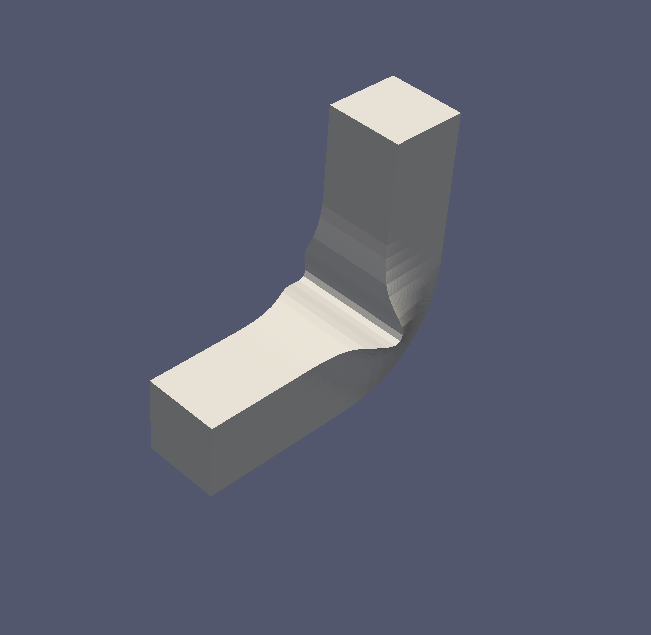
\includegraphics[width=8cm]{bend_result}
\centering
\end{figure}

Twist Deform Tool:
\begin{figure}[H]
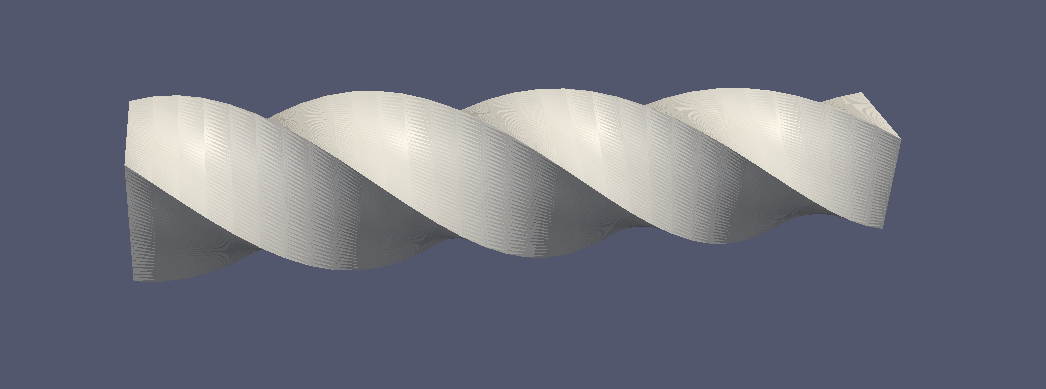
\includegraphics[width=8cm]{twist_result}
\centering
\end{figure}

\section{Appendix}
Caculate the Bend Deform Tool's angular velocity:
\begin{figure}[H]
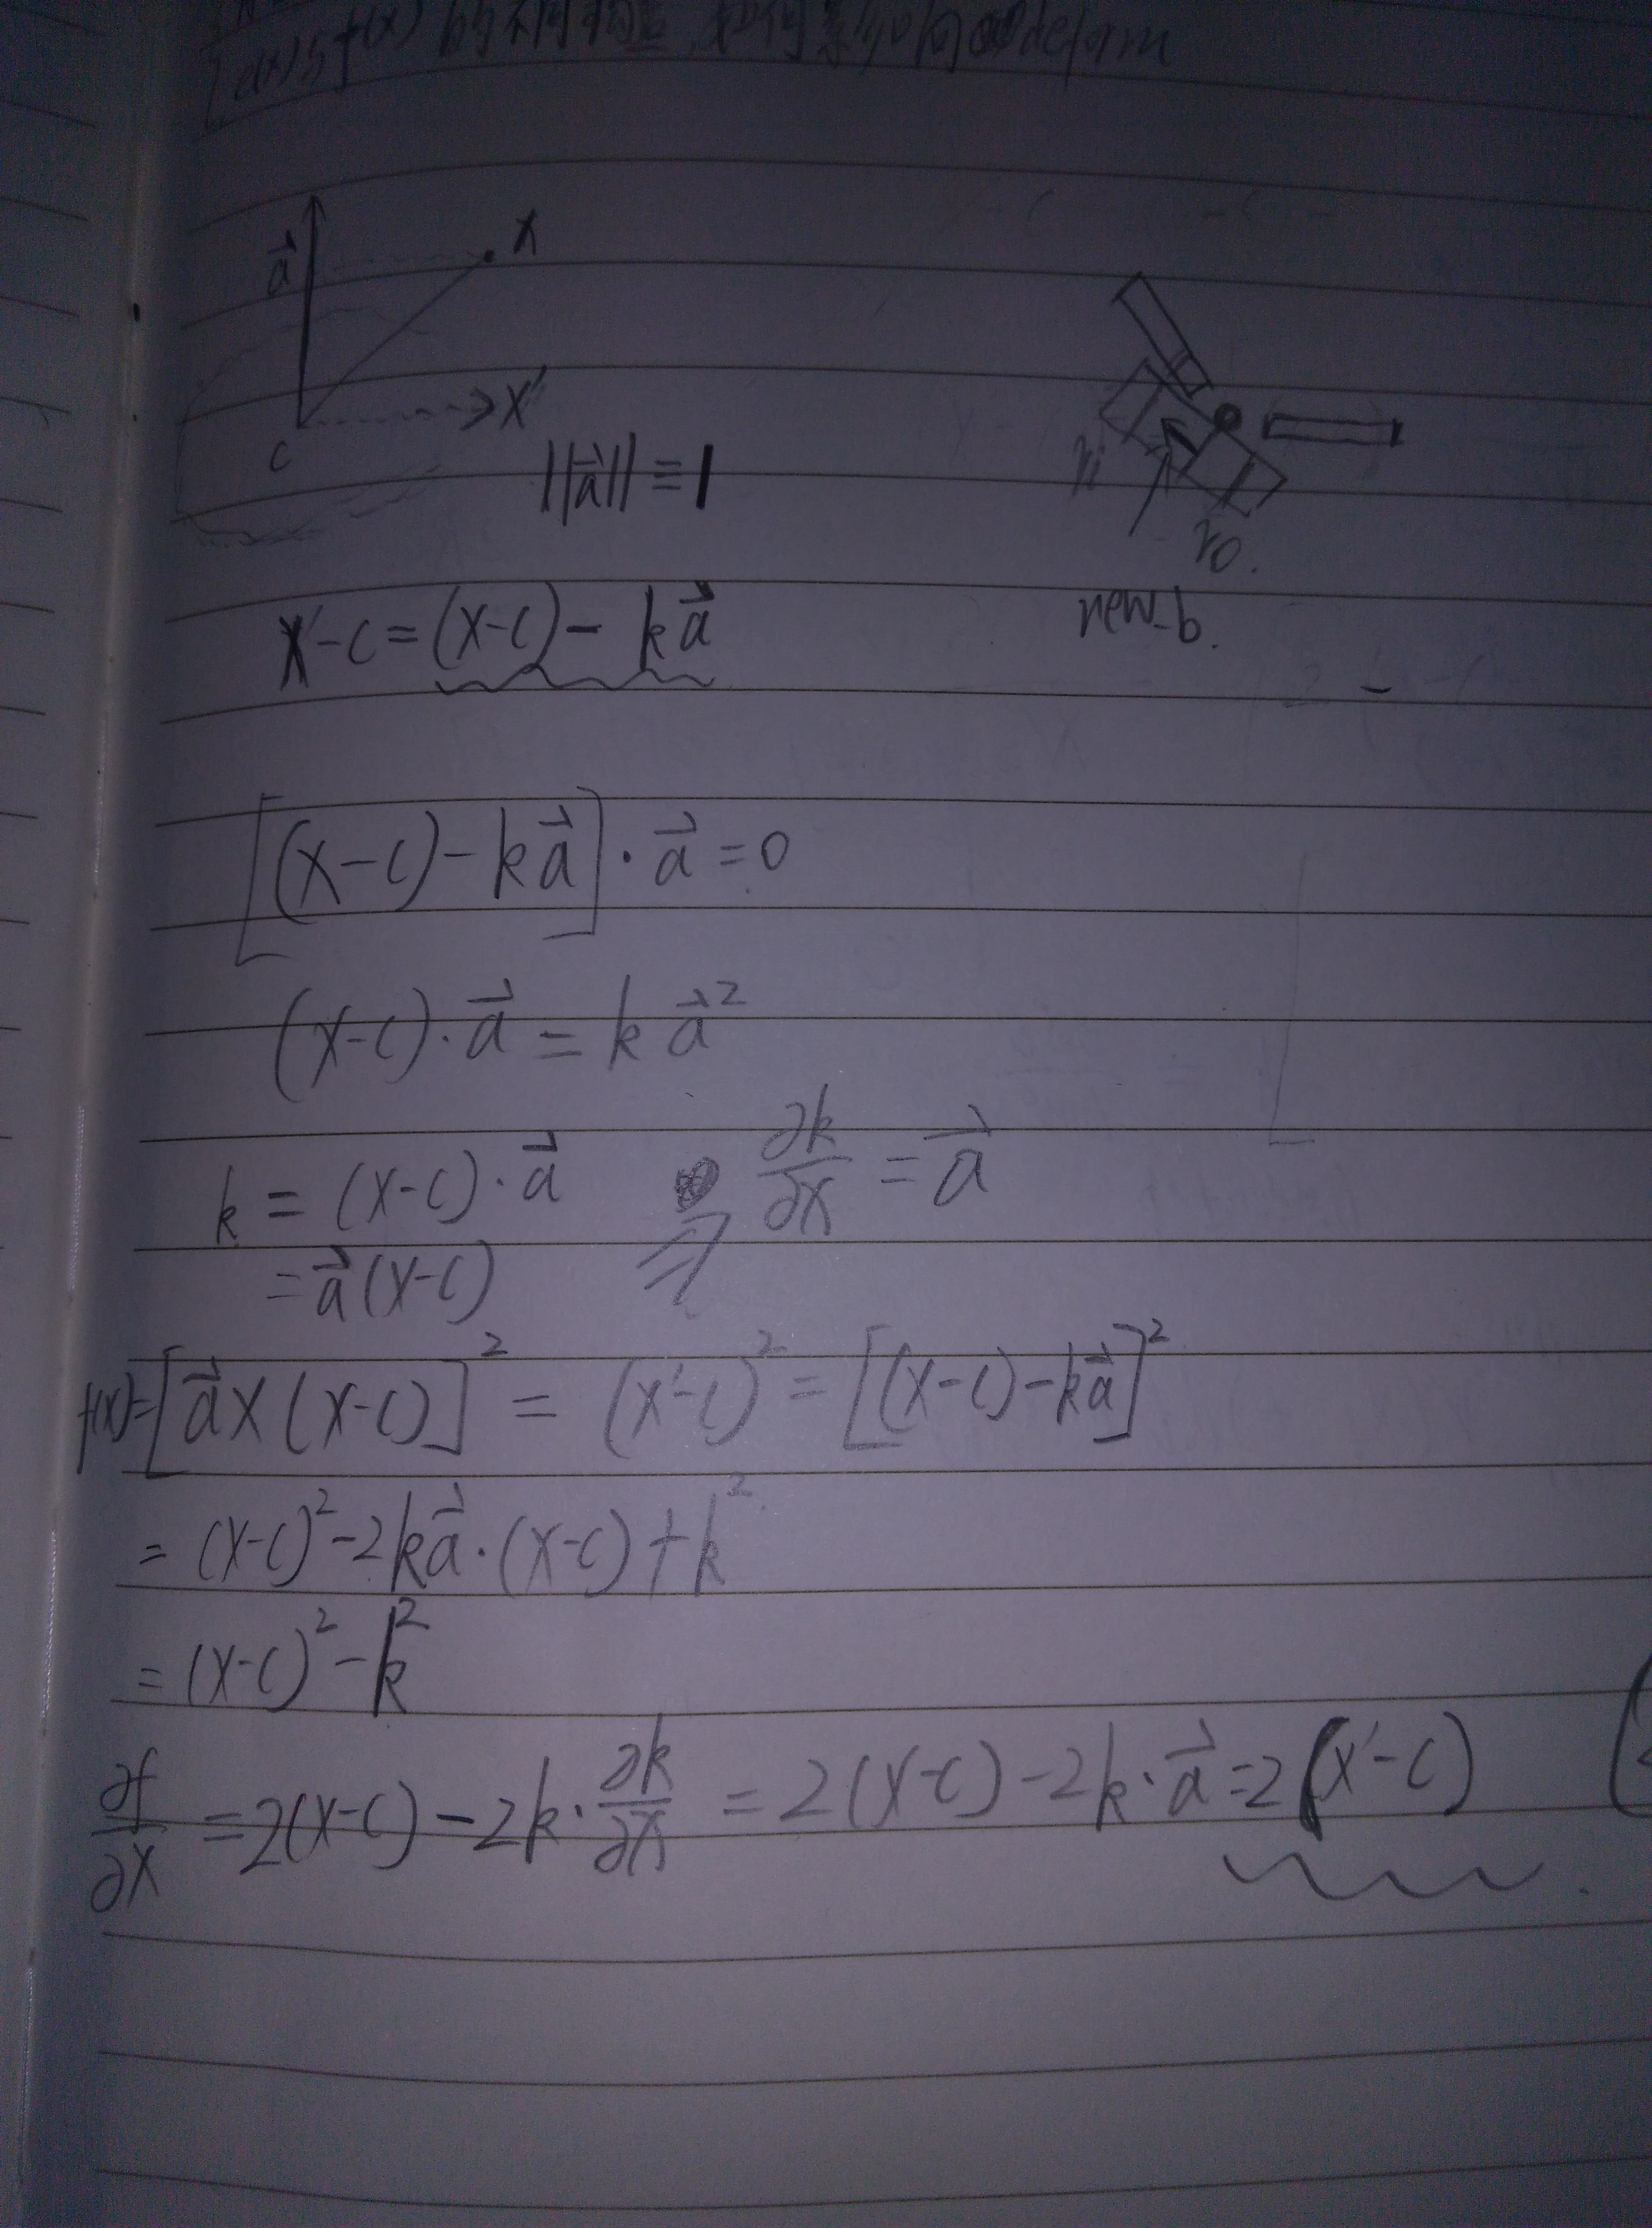
\includegraphics[width=8cm]{angular_velocity}
\centering
\end{figure}
Construct a scalar field let
\begin{equation}
  \nabla e = (\textbf{a} \cdot (x-c)) \textbf{a}
\end{equation}
then e(x) define as:
\begin{equation}
  \begin{aligned}
  e(x) &= \frac{a_0}{2}(x_0-c_0)^2 + \frac{a_1}{2}(x_1-c_1)^2 + \frac{a_2}{2}(x_2-c_2)^2 \\
  &+ a_0a_1(x_1-c_1)x_0 + a_0a_2(x_2-c_2)x_0+ a_1a_2(x_2-c_2)x_1\\
  &-a_1a_0c_0x_1-a_2a_0c_0x_2 - a_2a_1c_1x_2
  \end{aligned}
\end{equation}
%% \begin{equation}\label{eq:area}
%%   S = \pi r^2
%% \end{equation}
%% One can refer to equations like this: see equation (\ref{eq:area}). One can also
%% refer to sections in the same way: see section \ref{sec:nothing}. Or
%% to the bibliography like this: \cite{Cd94}.

%% \subsection{Subsection}\label{sec:nothing}

%% More text.

%% \subsubsection{Subsubsection}\label{sec:nothing2}

%% More text.

%% % Bibliography
%% %-----------------------------------------------------------------
%% \begin{thebibliography}{99}

%% \bibitem{Cd94} Author, \emph{Title}, Journal/Editor, (year)

%% \end{thebibliography}

\end{document}
